\chapter{Liquid Neural Network Design and Implementation}

\section{Design Overview}
This chapter outlines the implementation of the Liquid Neural Network (LNN) developed in PyTorch for sequential 2D time-series prediction. The architecture is based on the Liquid Time-Constant (LTC) neuron model, which simulates continuous-time dynamics through ordinary differential equations (ODEs) and shows properties of neural adaptability and temporal memory.

The aim of the implementation was to create a biologically-inspired, interpretable recurrent model with competitive performance on trajectory prediction tasks. Unlike conventional RNNs or LSTMs, the LNN is governed by time-continuous equations rather than discrete updates, providing finer control over neuronal dynamics.

\vspace{1em}
\noindent The following principles guided the design:
\begin{itemize}
    \item \textbf{Framework:} PyTorch was selected due to its flexible dynamic graph construction and ease of integrating custom layers with automatic differentiation.
    \item \textbf{Neuron Dynamics:} The neuron model was designed to emulate leaky integrate-and-fire (LIF) behaviour with added plasticity through modulated reversal potentials and conductances.
    \item \textbf{Time Unfolding:} Each forward pass of the LNN integrates over multiple internal time steps (ODE unfolds) to approximate the continuous-time solution, reflecting membrane voltage evolution.
    \item \textbf{Baseline Comparison:} To benchmark performance, identical training and evaluation protocols were implemented for alternative architectures (LSTM, TCN) using the same data.
\end{itemize}

The following sections document the architecture, neuron formulation, wiring strategy, training setup, and performance characteristics of the LNN.

\section{Wiring and Connectivity}
LNNs have a sparse and biologically motivated connectivity structure. To simulate the non-uniform and random nature of synaptic wiring observed in biological networks, a custom class named \texttt{RandomWiring} was implemented.

This class generates two adjacency matrices:
\begin{itemize}
    \item A \textbf{recurrent adjacency matrix} of shape $(n \times n)$ defining internal connections between neurons within the hidden layer.
    \item A \textbf{sensory adjacency matrix} of shape $(d_{\text{in}} \times n)$ which defines the input-to-hidden connectivity.
\end{itemize}
Each matrix contains continuous values sampled from a uniform distribution on $[0, 1]$, which are later used to create binary masks or to modulate weight strengths.

The \texttt{RandomWiring} class also generates reversal potentials: \texttt{erev} for neuron-neuron connections, and \texttt{sensory\_erev} for input-synapse connections. These potentials are initialised from a uniform range $[-0.2, 0.2]$ and are treated as fixed, non-learnable parameters.

The use of fixed sparse masks in the class emulate the limited number of active connections in real cortical microcircuits, enabling \textbf{biological plausibility}. In addition, each \textbf{randomised instantiation} of \texttt{RandomWiring} results in a different network topology, allowing stochastic variation in experiments.

Finally, the sensory and recurrent wiring are \textbf{decoupled}, to enable the model to explicitly distinguish between input-driven and internal dynamic behaviour.

Below is a simplified example of the \texttt{RandomWiring} class:
\begin{lstlisting}[language=Python, caption={Simplified RandomWiring class}]
class RandomWiring:
    def __init__(self, input_dim, output_dim, neuron_count):
        self.adjacency_matrix = np.random.uniform(0, 1, (neuron_count, neuron_count))
        self.sensory_adjacency_matrix = np.random.uniform(0, 1, (input_dim, neuron_count))
        
    def erev_initializer(self):
        return np.random.uniform(-0.2, 0.2, (neuron_count, neuron_count))

    def sensory_erev_initializer(self):
        return np.random.uniform(-0.2, 0.2, (input_dim, neuron_count))
\end{lstlisting}

\section{LTC Neuron Dynamics}
The core unit of the LNN is the \texttt{LIFNeuronLayer}, a custom PyTorch module that simulates the behaviour of leaky integrate-and-fire neurons (also known as liquid time-constant neurons). These neurons operate using a continuous-time dynamical model controlled by a first-order differential equation, capturing the evolution of membrane potentials in response to internal and external stimuli.

The model integrates over time using a discretised ODE solver implemented within the forward pass. Specifically, it unfolds the membrane update equation over a fixed number of steps (\texttt{ode\_unfolds}) using an Euler-like method.

\noindent The update rule is determined by the equation:

\begin{equation}
    \begin{aligned}
    v_i^{(t+1)} = \frac{1}{Z} \Bigg( 
    \softp(c_{m,i}) \cdot v_i^{(t)} + 
    \softp(g_{\text{leak},i}) \cdot V_{\text{leak},i} \\
    + \sum_j \underbrace{ \softp(w_{ij}) \cdot \sigma(v_j^{(t)}; \mu_{ij}, \sigma_{ij}) \cdot E_{\text{rev},ij} }_{\text{Recurrent synaptic current}} \\
    + \sum_k \underbrace{ \softp(w^{\text{sens}}_{ki}) \cdot \sigma(x_k; \mu^{\text{sens}}_{ki}, \sigma^{\text{sens}}_{ki}) \cdot E^{\text{sens}}_{\text{rev},ki} }_{\text{Sensory synaptic current}} 
    \Bigg)
    \end{aligned}
    \label{eq:v_update}
\end{equation}

\begin{equation}
Z = 
\softp(c_{m,i}) + 
\softp(g_{\text{leak},i}) +
\sum_j \softp(w_{ij}) \cdot \sigma(v_j^{(t)}; \mu_{ij}, \sigma_{ij}) +
\sum_k \softp(w^{\text{sens}}_{ki}) \cdot \sigma(x_k; \mu^{\text{sens}}_{ki}, \sigma^{\text{sens}}_{ki}) + \varepsilon
\label{eq:v_update_denominator}
\end{equation}

\noindent where:
\begin{itemize}
    \item \( \softp(\cdot) = \text{Softplus}(\cdot) = \log(1 + e^{(\cdot)}) \): nonlinearity ensuring positivity of weights and conductances
    \item $v_i^{(t)}$: membrane potential of neuron $i$ at ODE step $t$
    \item $x_k$: sensory input from dimension $k$
    \item $\sigma(v; \mu, \sigma) = \text{sigmoid}(\sigma (v - \mu))$: synaptic activation function
    \item $w_{ij}$: weight from neuron $j$ to neuron $i$ (recurrent)
    \item $w^{\text{sens}}_{ki}$: weight from input $k$ to neuron $i$ (sensory)
    \item $\mu$, $\sigma$: learnable sigmoid parameters (mean and scale)
    \item $E_{\text{rev}}$, $E^{\text{sens}}_{\text{rev}}$: synaptic reversal potentials
    \item $V_{\text{leak}}$: fixed leak reversal potential
    \item $c_m$, $g_{\text{leak}}$: learnable membrane capacitance and leak conductance
    \item $\varepsilon$: small constant for numerical stability
\end{itemize}

\noindent This formulation reflects the true internal update logic of the \texttt{LIFNeuronLayer} implementation, where each neuron's potential evolves through a biophysically inspired ODE governed by input-specific and recurrent dynamics.

\begin{figure}[H]
    \centering
    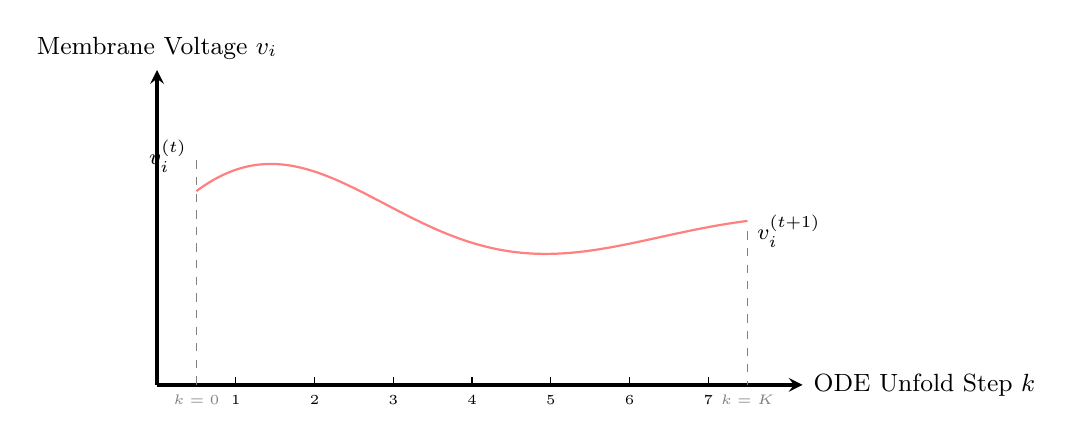
\begin{tikzpicture}[
        axis/.style={very thick, ->, >=stealth},
        voltage/.style={draw=red!50, thick, smooth},
        time/.style={font=\small},
        every node/.style={font=\small}
    ]

    % Axes
    \draw[axis] (0,0) -- (8.2,0) node[right] {ODE Unfold Step $k$};
    \draw[axis] (0,0) -- (0,4.0) node[above] {Membrane Voltage $v_i$};

    % Tick labels (k)
    \foreach \x in {1,2,...,7}
        \draw (\x,0) -- (\x,0.1) node[below=3pt] {\tiny $\x$};

    % Voltage trace (stylised)
    \draw[voltage, domain=0.5:7.5, samples=100] plot (\x, {2 + 1.2*sin(deg(0.9*\x))*exp(-0.25*\x)});

    % Annotate starting voltage
    \draw[dashed, gray] (0.5,2.85) -- (0.5,0) node[below] {\tiny $k=0$};
    \node at (0.5,2.9) [left, font=\footnotesize] {$v_i^{(t)}$};

    % Annotate final voltage
    \draw[dashed, gray] (7.5,1.95) -- (7.5,0) node[below] {\tiny $k=K$};
    \node at (7.5,1.95) [right, font=\footnotesize] {$v_i^{(t+1)}$};

    \end{tikzpicture}
    \caption{Illustrative internal membrane voltage trace across $K$ ODE unfolding steps for a single neuron. This entire graph represents the internal dynamics used to compute $v_i^{(t+1)}$ from $v_i^{(t)}$, in a single timestep.}
    \label{fig:lif_voltage_evolution}
\end{figure}

Unlike traditional RNNs or LSTMs, which update their hidden state in a single discrete operation per time step, Liquid Time-Constant neurons simulate fine-grained membrane voltage dynamics by performing multiple internal updates within each input timestep. This behaviour is governed by the discretised solution of the differential equations (see Equation~\ref{eq:v_update} and Equation~\ref{eq:v_update_denominator}).

At each unfolding step, the membrane potential is updated using a softplus-modulated combination of capacitive memory, leak current, and synaptic input currents. These updates reflect physical dynamics such as charging, leak, and synaptic integration, enabling the neuron to adaptively integrate information over sub-timestep resolution. The final membrane voltage $v_i^{(t+1)}$ is the result of this integration process and is passed forward in time.

This is different from gated memory in LSTMs, which uses learnable gates and affine transformations, or temporal convolutions in TCNs, which apply fixed receptive filters. Instead, the LTC neuron learns dynamic temporal behaviour through time constants and nonlinear integration, making it particularly suited to tasks that require fine temporal resolution and state-dependent transitions.

\vspace{1em}
\noindent \textbf{Implementation Details:}
\begin{itemize}
    \item \textbf{Learnable Parameters:} All biophysical constants (capacitance, leak conductance, reversal potentials, synaptic weights) are learnable, providing flexibility in dynamic behaviour.
    \item \textbf{Softplus Regularisation:} Weights and conductances are passed through \texttt{Softplus} to enforce positivity while allowing gradients to flow smoothly during training.
    \item \textbf{ODE Unfolding:} The number of internal solver steps is fixed (\texttt{ode\_unfolds} = 12) to balance numerical precision with computational cost.
    \item \textbf{Sparsity Masks:} Both recurrent and sensory activations are element-wise masked using the adjacency matrices from \texttt{RandomWiring}, enforcing fixed sparsity throughout training.
\end{itemize}

\noindent Below is the ODE solver implementation within the \texttt{LIFNeuronLayer} class:
\begin{lstlisting}[language=Python, caption={Simplified LTC neuron forward method}]
def ode_solver(self, inputs, state, elapsed_time):
    v_pre = state
    for _ in range(self.ode_unfolds):
        synaptic_input = compute_synaptic_activation(v_pre)
        numerator = self.cm * v_pre + self.gleak * self.vleak + synaptic_input
        denominator = self.cm + self.gleak + synaptic_conductance
        v_pre = numerator / (denominator + self.epsilon)
    return v_pre
\end{lstlisting}
This allows neurons to respond to both present input and also to their internal temporal dynamics, mimicking continuous-time memory traces observed in biological neurons.

\begin{figure}[H]
    \centering
    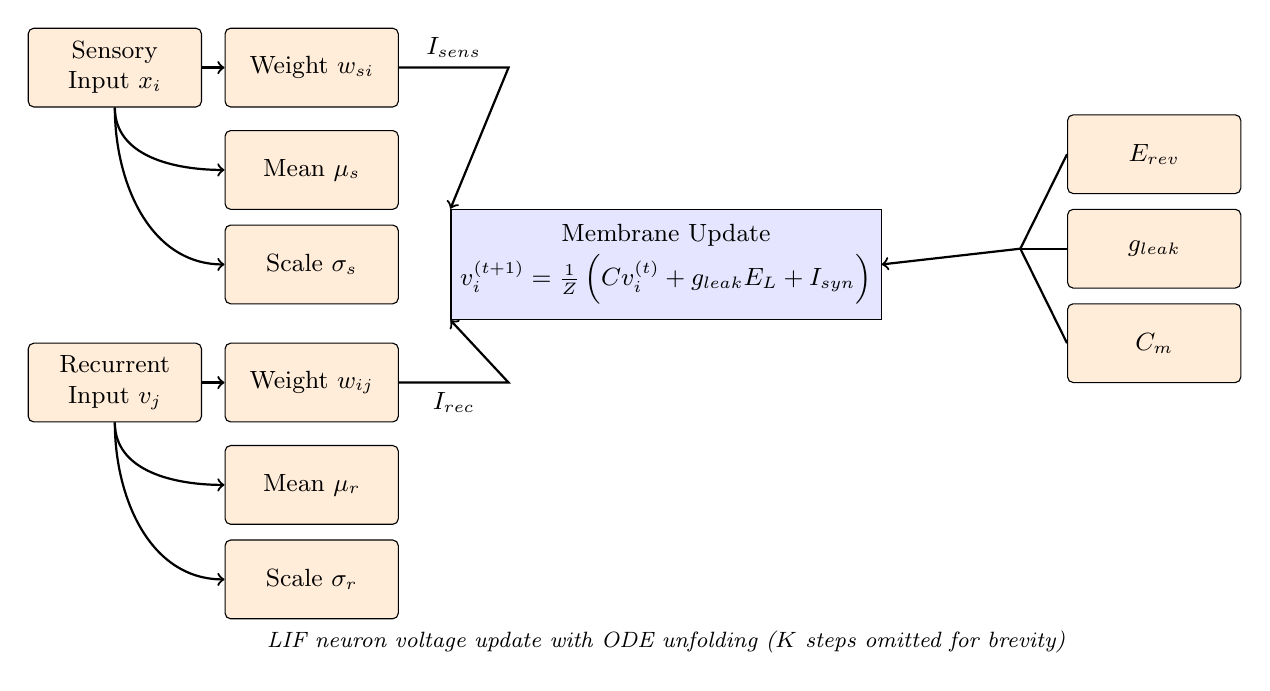
\begin{tikzpicture}[
        box/.style={draw, minimum height=1.4cm, minimum width=2.8cm, align=center, fill=blue!10},
        label/.style={font=\footnotesize\itshape},
        param/.style={draw, rounded corners=2pt, fill=orange!15, minimum height=1cm, minimum width=2.2cm, align=center},
        arrow/.style={->, thick},
        line/.style={-, thick},
        every node/.style={font=\small}
    ]
    
    % Sensory Input
    \node[param] (sens_input) at (-5, 3.5) {Sensory\\Input $x_i$};
    \node[param] (sens_w) at (-2.5, 3.5) {Weight $w_{si}$};
    \node[param] (sens_mu) at (-2.5, 2.2) {Mean $\mu_s$};
    \node[param] (sens_sigma) at (-2.5, 1.0) {Scale $\sigma_s$};
    \draw[arrow] (sens_input) -- (sens_w);
    \draw[arrow] (sens_input.south) to[out=270,in=180] (sens_mu.west);
    \draw[arrow] (sens_input.south) to[out=270,in=180] (sens_sigma.west);
    
    % Recurrent Input
    \node[param] (rec_input) at (-5, -0.5) {Recurrent\\Input $v_j$};
    \node[param] (rec_w) at (-2.5, -0.5) {Weight $w_{ij}$};
    \node[param] (rec_mu) at (-2.5, -1.8) {Mean $\mu_r$};
    \node[param] (rec_sigma) at (-2.5, -3.0) {Scale $\sigma_r$};
    \draw[arrow] (rec_input) -- (rec_w);
    \draw[arrow] (rec_input.south) to[out=270,in=180] (rec_mu.west);
    \draw[arrow] (rec_input.south) to[out=270,in=180] (rec_sigma.west);
    
    % Membrane Update Box
    \node[box] (voltage) at (2, 1.0) {Membrane Update\\[2pt] $v_i^{(t+1)} = \frac{1}{Z} \left(C v_i^{(t)} + g_\text{leak} E_L + I_{\text{syn}} \right)$};
    
    % Inputs into Membrane Box
    \draw[arrow] (sens_w.east) -- (0, 3.5) node[midway, above] {$I_{\text{sens}}$} -- (voltage.north west);
    \draw[arrow] (rec_w.east) -- (0, -0.5) node[midway, below] {$I_{\text{rec}}$} -- (voltage.south west);
    
    % Right-side parameters
    \node[param] (erev) at (8.2, 2.4) {$E_\text{rev}$};
    \node[param] (gleak) at (8.2, 1.2) {$g_\text{leak}$};
    \node[param] (cm) at (8.2, 0.0) {$C_m$};
    
    % Junction point
    \coordinate (rightjunction) at (6.5, 1.2);
    
    % Connect parameters to junction (no arrowheads)
    \draw[line] (erev.west) -- (rightjunction);
    \draw[line] (gleak.west) -- (rightjunction);
    \draw[line] (cm.west) -- (rightjunction);
    
    % Final arrow into voltage box
    \draw[arrow] (rightjunction) -- (voltage.east);
    
    % Caption
    \node[label] at (2, -3.8) {LIF neuron voltage update with ODE unfolding ($K$ steps omitted for brevity)};
    
    \end{tikzpicture}
    \caption{Internal structure of a single LIF neuron used in the Liquid Time-Constant Network. Inputs undergo non-linear transformations based on trainable $\mu$ and $\sigma$, and the resulting activations are integrated using biophysical parameters (leak conductance $g_\text{leak}$, membrane capacitance $C_m$, and reversal potentials $E_\text{rev}$).}
    \label{fig:lif_neuron_detailed}
\end{figure}


\section{Network Architecture}
The full LNN is constructed by embedding the LTC neuron layer inside a recurrent wrapper, implemented as a custom \texttt{LTCRNN} module. This wrapper sequentially passes each time step of the input through the same \texttt{LIFNeuronLayer}, maintaining a hidden state that evolves over time. The resulting structure can be viewed as a biologically grounded alternative to traditional RNN cells.

The architecture accepts an input tensor of shape $(B, T, d_{\text{in}})$, where $B$ is the batch size, $T$ is the sequence length, and $d_{\text{in}}$ is the input dimension (two in this case, corresponding to 2D spatial coordinates). For each time step $t$, the neuron layer receives the $t$-th slice of the sequence and updates the hidden state, generating a predicted output of shape $(B, T, d_{\text{out}})$.

\subsection*{Design Considerations}
While designing the LTCRNN architecture, there were several key design decisions made. The hidden state dimensionality (i.e. number of LTC neurons) defined the model capacity; lower values reduce overfitting risk and improve computational efficiency at the cost of limited expressiveness. In addition, the voltage traces themselves are treated as predictions instead of applying a separate output layer. This means membrane state is directly used as a continuous output signal. To maximise efficiency (and GPU parallelism) of tensor operations during training/inference, all sequences are processed in batch-major form (following PyTorch convention).

\noindent Below is a simplified version of this architecture:
\begin{lstlisting}[language=Python, caption={Structure of the LTCRNN module}]
class LTCRNN(nn.Module):
    def __init__(self, wiring, input_dim, hidden_dim, output_dim):
        self.cell = LIFNeuronLayer(wiring)
        ...
        
    def forward(self, inputs):
        batch_size, seq_len, _ = inputs.size()
        states = torch.zeros(batch_size, self.hidden_dim)
        outputs = []
        for t in range(seq_len):
            out, states = self.cell(inputs[:, t, :], states)
            outputs.append(out)
        return torch.stack(outputs, dim=1)
\end{lstlisting}

The design maintains a clear distinction between the continuous-time neuronal dynamics and the sequence-level integration logic. Thus, it is both modular and biologically interpretable, and compatible with standardised modern deep learning tools.

\begin{figure}[H]
    \centering
    \begin{tikzpicture}[
        neuron/.style={circle, draw=black, fill=blue!15, minimum size=1.2cm},
        lif/.style={rectangle, draw=black, rounded corners=2pt, fill=red!15, minimum height=1.2cm, minimum width=1.8cm},
        input/.style={draw=black, fill=orange!15, minimum width=1.2cm, minimum height=0.7cm, text centered},
        output/.style={draw=black, fill=green!20, minimum width=1.6cm, minimum height=0.8cm, text centered},
        arrow/.style={->, thick},
        every node/.style={font=\small}
    ]

    % Input block
    \node[input] (input1) at (0,1.5) {$x_1$};
    \node[input] (input2) at (0,0.5) {$x_2$};
    \node at (0,-0.2) {$\vdots$};
    \node[input] (inputm) at (0,-1.2) {$x_m$};

    \node[draw=blue!40, thick, rounded corners=3pt, fit=(input1)(input2)(inputm), inner sep=5pt, label=above:Input Sequence] (inputbox) {};

    % Sensory Projection
    \node at (2.3, 0.1) {\textbf{Sensory Projections}};
    \draw[arrow] (input1) -- (2,1.5);
    \draw[arrow] (input2) -- (2,0.5);
    \draw[arrow] (inputm) -- (2,-1.2);
    \node at (2,-0.2) {$\vdots$};

    % LIF Neuron Layer (Liquid Layer)
    \node[lif] (lif1) at (4,2.0) {LIF$_1$};
    \node[lif] (lif2) at (4,0.8) {LIF$_2$};
    \node at (4,-0.2) {$\vdots$};
    \node[lif] (lifn) at (4,-1.5) {LIF$_n$};
    
    \node[draw=black, thick, dashed, fit=(lif1)(lif2)(lifn), inner sep=10pt, label=above:Liquid Layer] (liquidbox) {};

    % Internal recurrent wiring (sparse)
    \draw[arrow, bend left=20] (lif1) to (lif2);
    \draw[arrow, bend left=30] (lif2) to (lifn);
    \draw[arrow, bend left=30] (lifn) to (lif1);

    % Sensory to Liquid
    \draw[arrow] (2,1.5) -- (lif1.west);
    \draw[arrow] (2,0.5) -- (lif2.west);
    \draw[arrow] (2,-1.2) -- (lifn.west);

    % Output Projection (Readout)
    \node[output] (out) at (7,0) {Output};

    \draw[arrow] (lif1.east) -- (out);
    \draw[arrow] (lif2.east) -- (out);
    \draw[arrow] (lifn.east) -- (out);

    % Labels
    \node at (4.2,-2.3) {\footnotesize ODE Solver (Unfolded $K$ steps)};
    \node at (7.3,-0.8) {\footnotesize Readout Layer};

    \end{tikzpicture}
    \caption{Architecture of the Liquid Time-Constant Network (LNN). Inputs project through learned sensory filters to a sparsely recurrent Liquid Layer of LIF neurons. Dynamics are integrated using an internal ODE solver with unfolding. Final outputs are read from a low-dimensional projection.}
    \label{fig:lnn_architecture}
\end{figure}


\section{Training Configuration (and dataset)}
The LNN was trained on a synthetic 2D spiral trajectory dataset, chosen for its smooth temporal structure and nonlinearity. Each data point consists of an $(x, y)$ coordinate, and the model's aim is to predict the next point in the sequence (given a fixed-length input window). The 'sequential' nature of the task makes it well-suited for testing temporal memory and continuous dynamics.

The synthetically-generated dataset ensured control over noise and resolution, which allowed clearer attribution of error sources to model limitations rather than data irregularities.

A supervised learning approach was used; inputs and targets were created by shifting a sliding window of length $T = 3$ over the full spiral. The small sequence length was chosen to reduce training complexity while still allowing temporal dependencies to be captured. Each input sequence of three time steps was paired with the corresponding next three steps as the target output.

The dataset was split into training and validation sets, with the training set containing 80\% of the data and the validation set containing 20\%. This split was randomised to ensure that the model generalised well to unseen data.

\subsubsection*{Data Preprocessing}
\begin{itemize}
    \item All inputs were standardised using the training set mean and standard deviation.
    \item Targets were normalised in the same way to preserve scale consistency.
    \item The spiral dataset was generated programmatically with adjustable number of points and turns.
\end{itemize}

subsubsection*{Training Parameters}
Mean Squared Error (\texttt{nn.MSELoss()}) was used to penalise deviations from the ground truth trajectory. Adam was chosen as the optimiser due to its fast convergence and robustness to parameter scaling, with a learning rate of 0.005. The model was trained for 2000 epochs, with periodic visual evaluation every 100 epochs. Input sequences were split into overlapping windows and grouped into batches of size 32, allowing efficient GPU utilisation while preserving temporal continuity. A random 80/20 train-validation split was applied, with shuffling to prevent memorisation of input order.

Below is the training process implementation:
\begin{lstlisting}[language=Python, caption={Simplified training loop for the LNN}]
for epoch in range(num_epochs):
    lnn_model.train()
    total_loss = 0
    for x_batch, y_batch in zip(input_batches, target_batches):
        optimizer.zero_grad()
        outputs = lnn_model(x_batch)
        loss = criterion(outputs, y_batch)
        loss.backward()
        optimizer.step()
        total_loss += loss.item()
\end{lstlisting}

The training loop includes evaluation checkpoints where predicted trajectories are plotted and compared to ground truth. These visualisations provided insights into convergence behaviour, beyond scalar loss values.

\section{Training Behaviour}
Throughout training, model performance was monitored both quantitatively (via validation loss) and qualitatively (through trajectory plots), every 100 epochs.

\noindent The main trends observed during training were:
\begin{itemize}
    \item Loss decreased steadily in early epochs, with diminishing returns as training progressed.
    \item In some cases, small fluctuations in validation loss were observed, likely due to the non-convexity of the parameter landscape and the biological variability induced by random wiring.
    \item Visual predictions of the trajectory showed clear improvement over time. Early predictions were coarse approximations, while later epochs gave smoother and more accurate predictions.
\end{itemize}

\subsection*{Trajectory Loss Curves}
To evaluate the model's learning progress and generalisation, we record the full-sequence mean squared error (MSE) first on the entire spiral sequence (which contains the training datapoints and the held-out validation datapoints), and then on a separate unseen evaluation spiral, at each epoch. Rather than separately plotting training and validation loss — which are contiguous segments of the same spiral trajectory, they are treated as a single sequence. This is because temporal continuity is essential in modelling dynamical systems. This avoids misleading interpretations that might arise from artificial segmentation of a naturally evolving system.

The following plots illustrates training and validation behaviour over time (the second is zoomed to highlight differences between the training/validation spiral and evaluation spiral):

\begin{figure}[H]
    \centering
    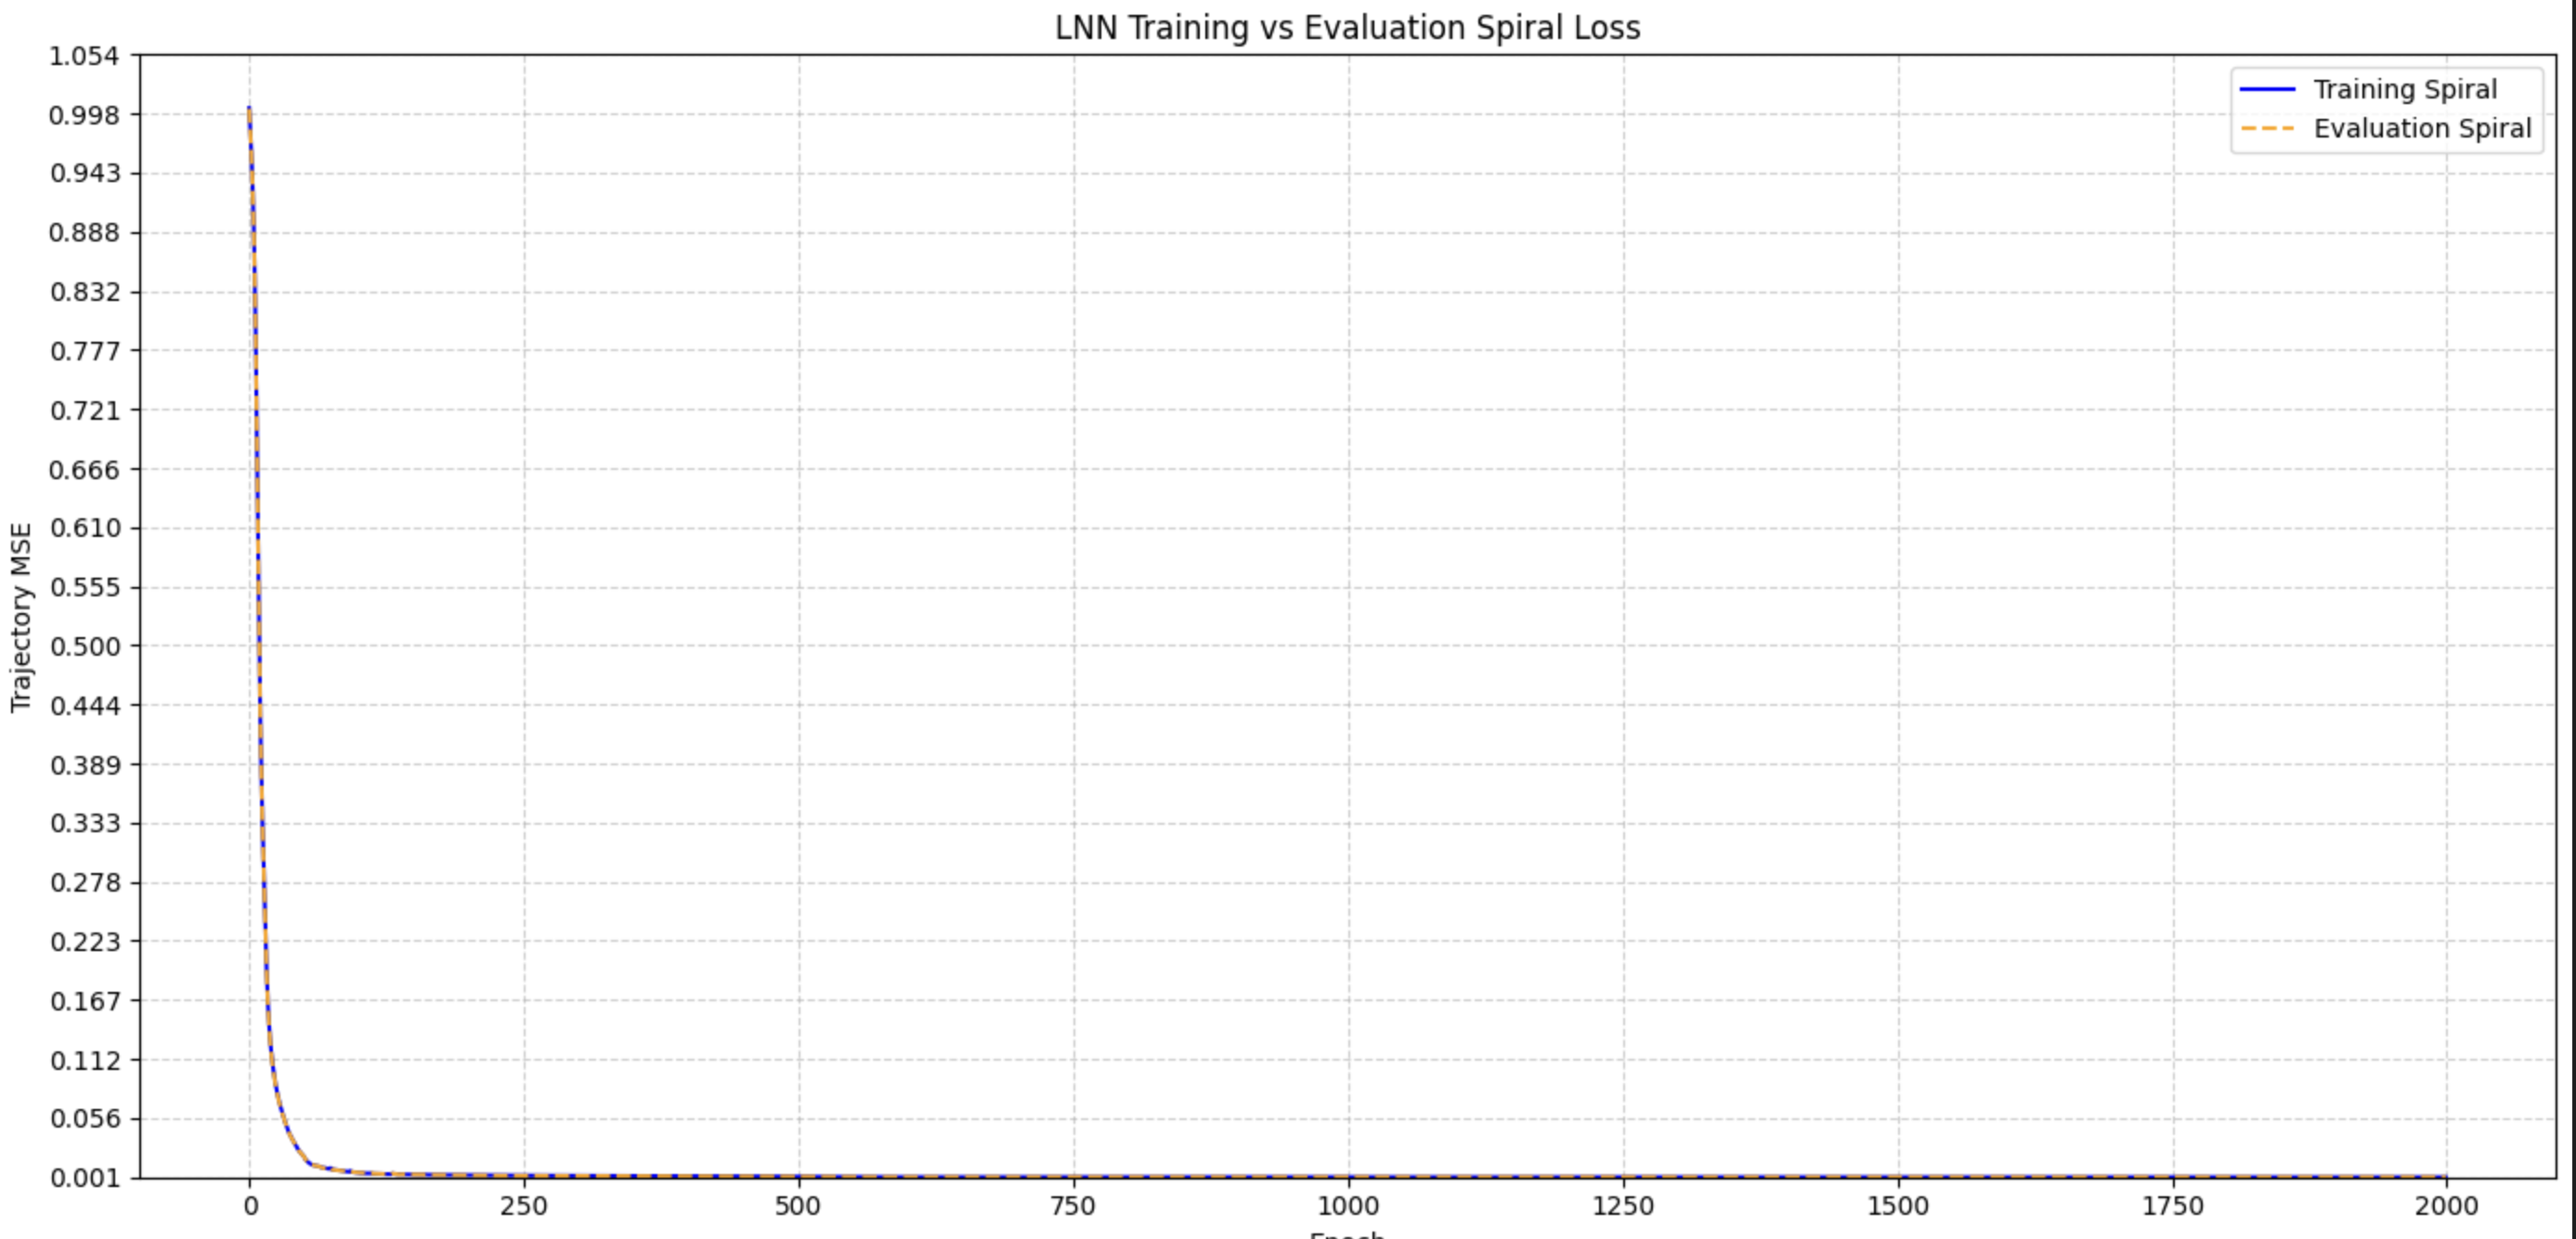
\includegraphics[width=0.8\linewidth]{img/lnn_loss_curve.png}
    \caption{Training and validation loss over epochs.}
    \label{fig:lnn_loss}
\end{figure}

\begin{figure}[H]
    \centering
    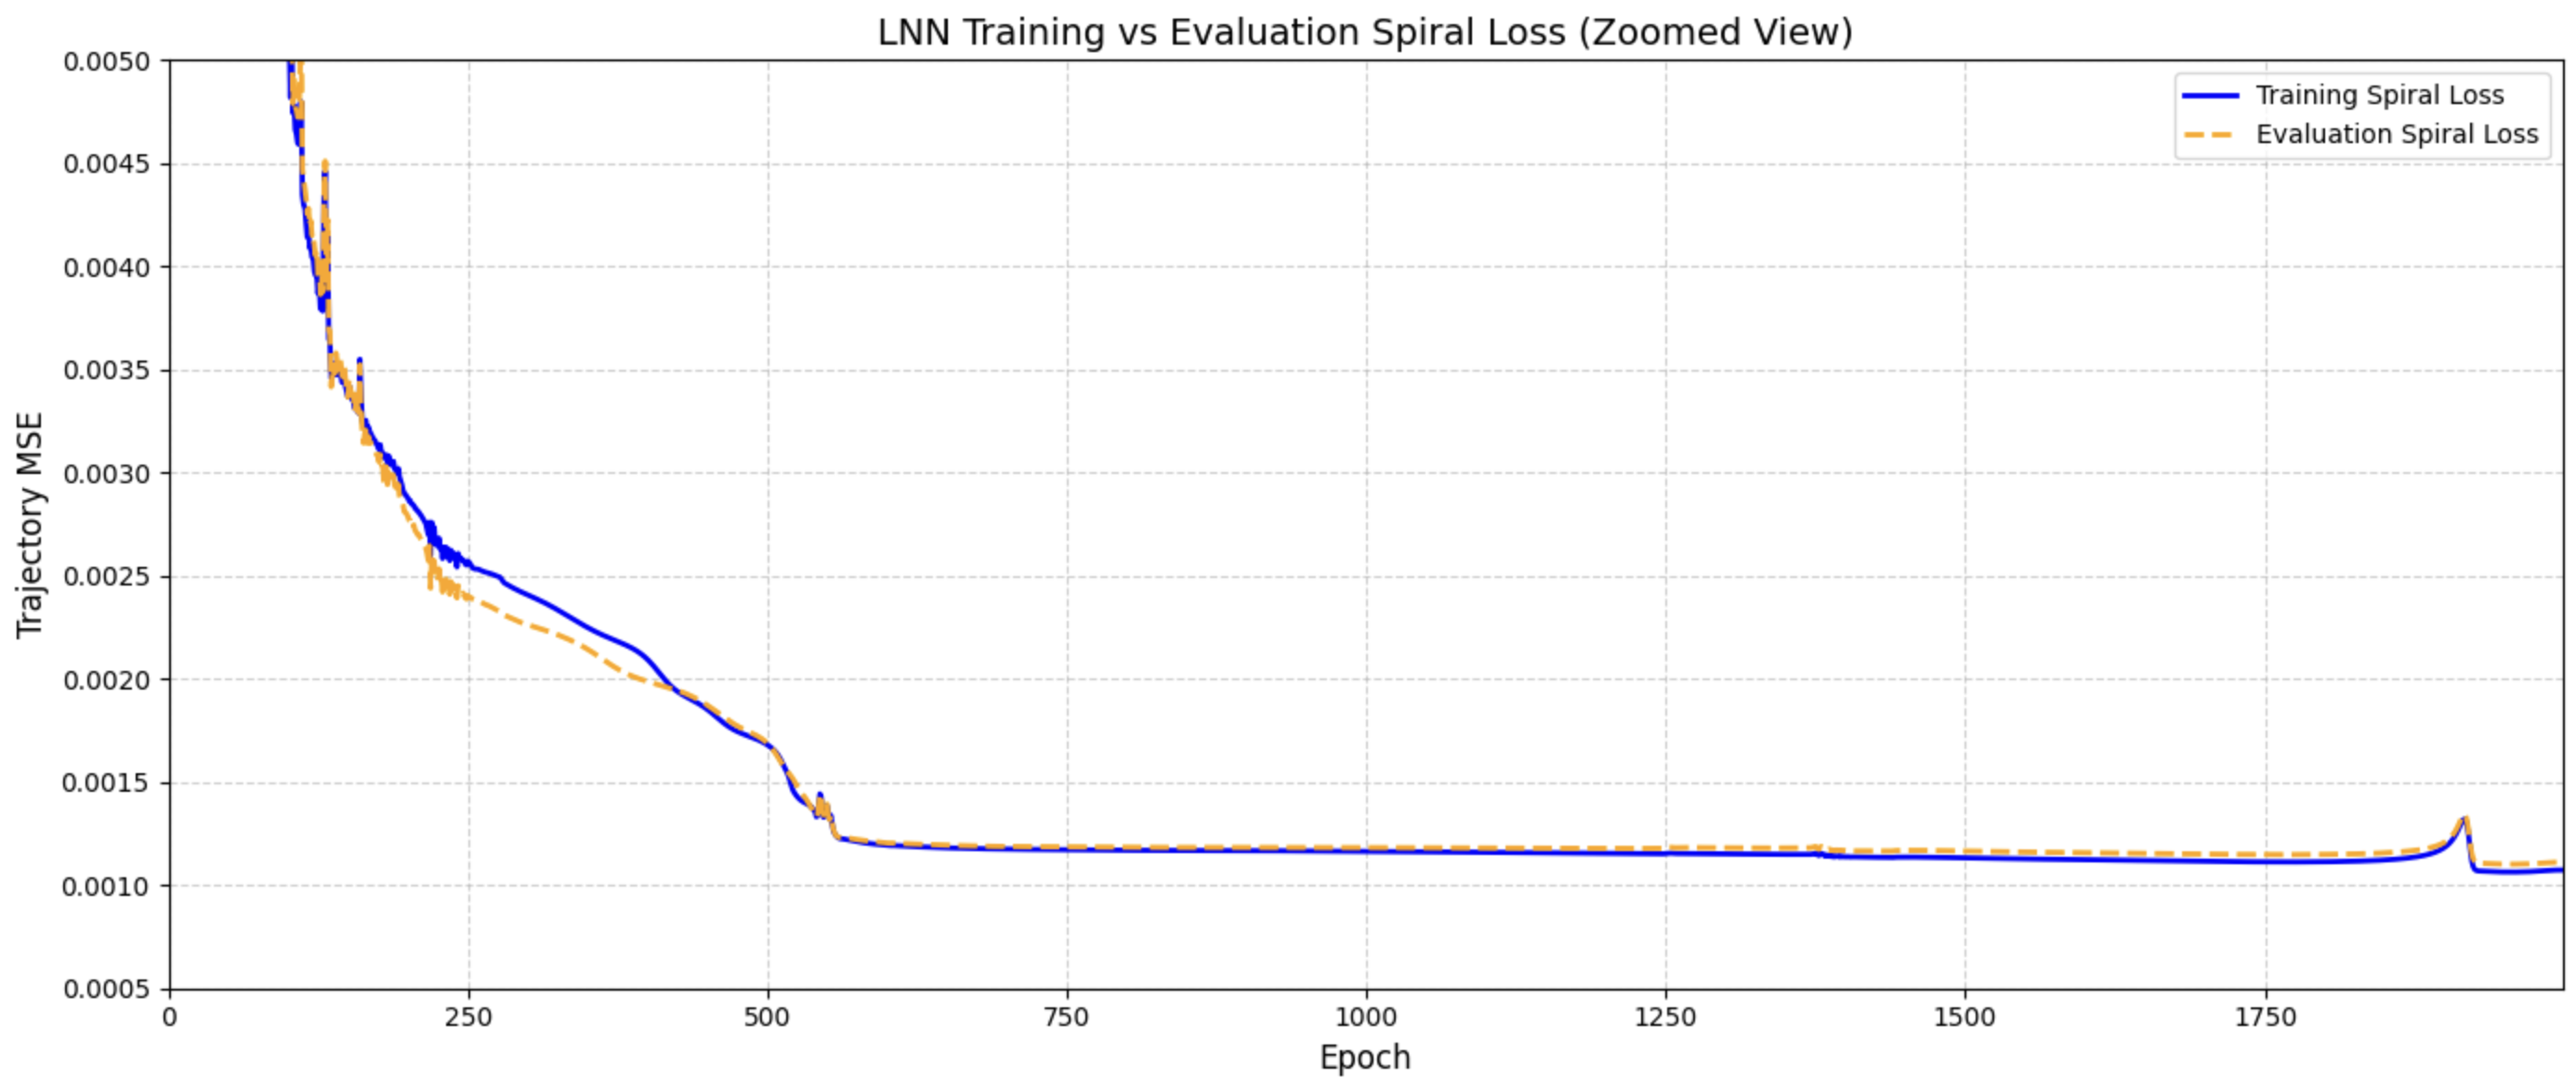
\includegraphics[width=0.8\linewidth]{img/lnn_loss_curve_zoomed.png}
    \caption{Training and validation loss over epochs (zoomed).}
    \label{fig:lnn_loss_zoomed}
\end{figure}

Early in training, both curves decrease rapidly, suggesting that the model learns the underlying structure efficiently. As training proceeds, the two curves converge, with the evaluation spiral maintaining a slightly higher loss, indicating some generalisation gap but also demonstrating stable extrapolation beyond the training path. Importantly, neither curve exhibits significant divergence or overfitting behaviour, which supports the robustness and consistency of the trained model.

\subsection*{Qualitative Evaluation}
Visually, the predicted path over time showed that the LNN was able to maintain smooth curvature and approximate the rotational dynamics of the spiral without overshooting or excessive lag. This was true even on validation data not seen during training. 

\begin{figure}[H]
    \centering
    \begin{subfigure}[b]{0.45\linewidth}
        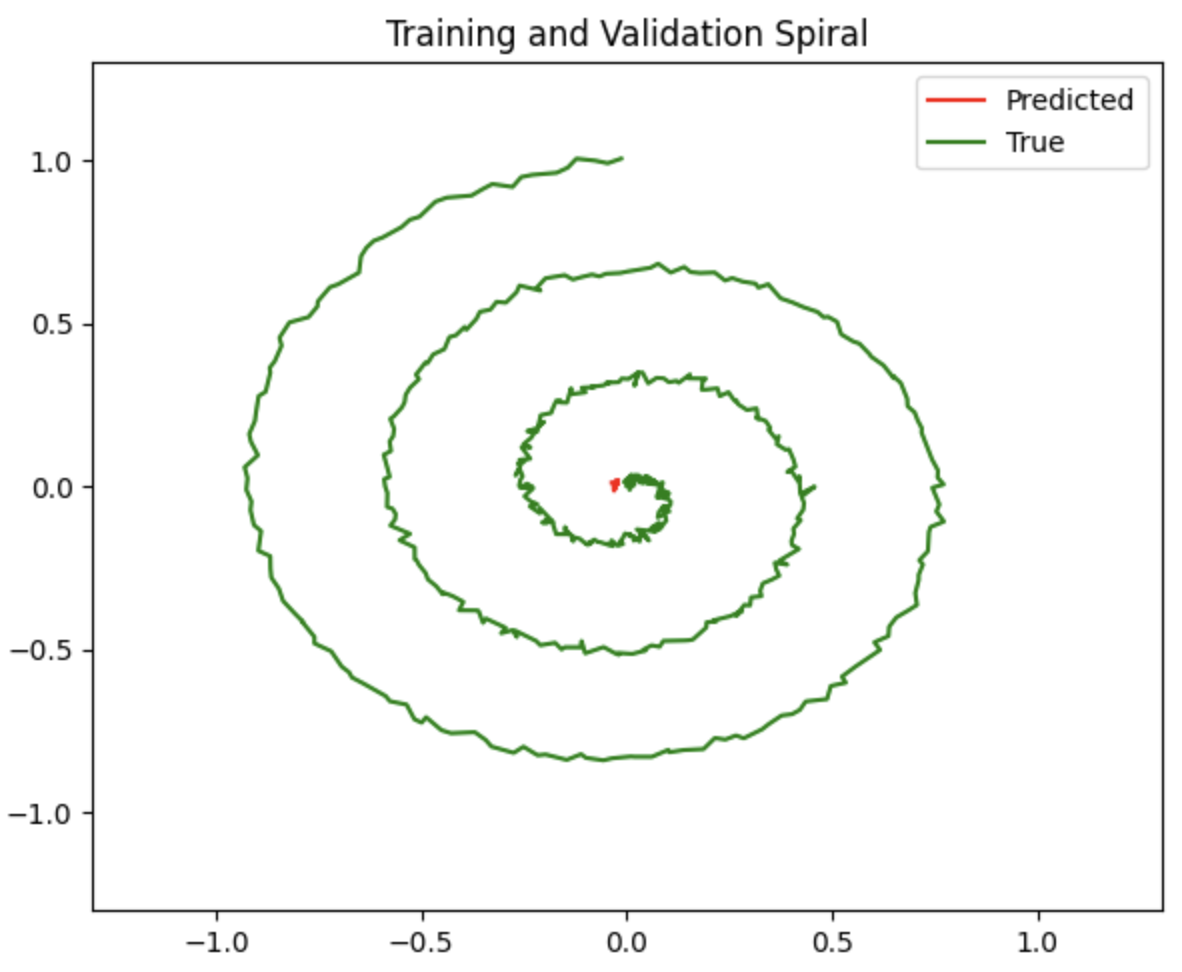
\includegraphics[width=\linewidth]{img/lnn_training_validation_spiral_epoch_1.png}
        \caption{Epoch 1}
        \label{fig:lnn_training_validation_spiral_epoch_1}
    \end{subfigure}
    \hfill
    \begin{subfigure}[b]{0.45\linewidth}
        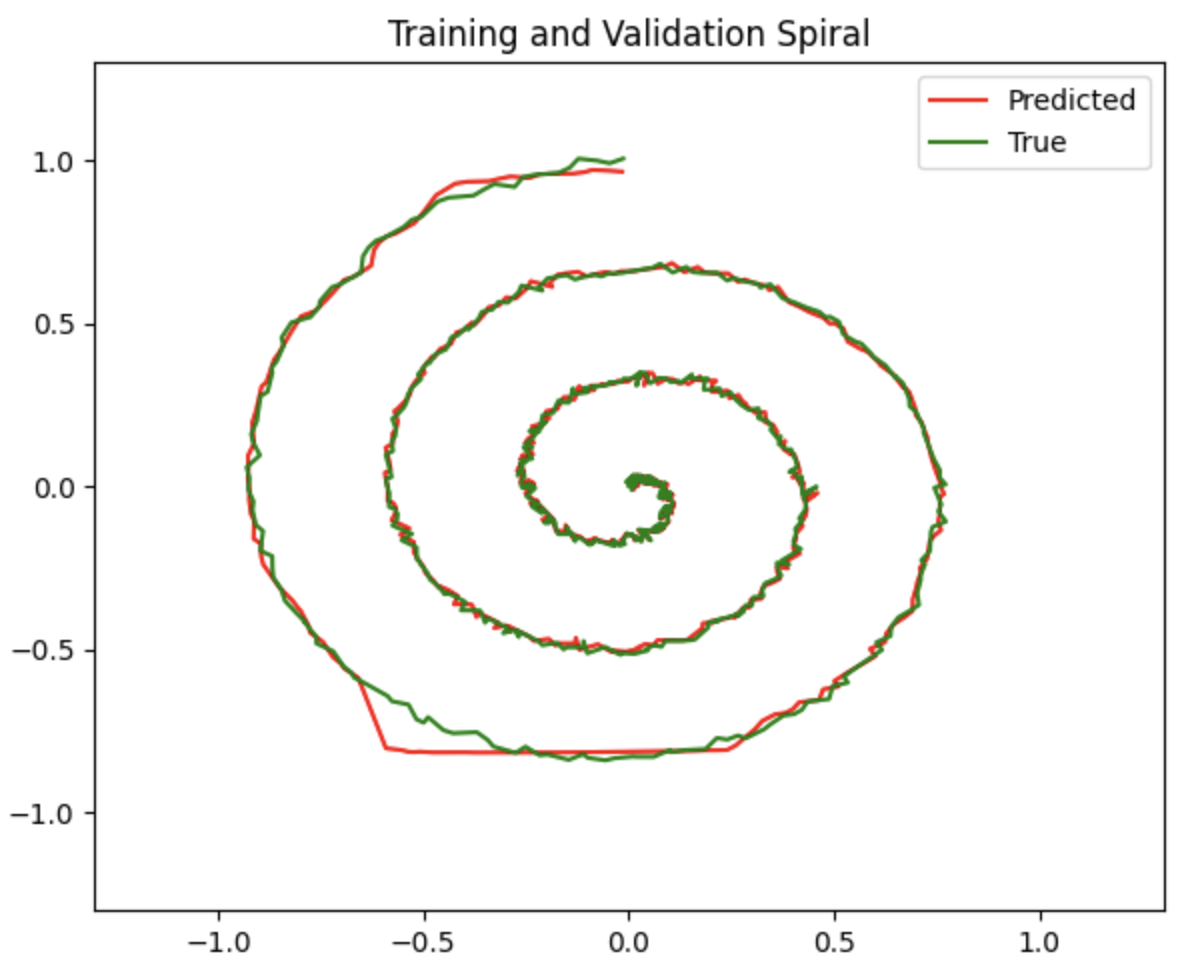
\includegraphics[width=\linewidth]{img/lnn_training_validation_spiral_epoch_400.png}
        \caption{Epoch 400}
        \label{fig:lnn_training_validation_spiral_epoch_400}
    \end{subfigure}
    \vskip\baselineskip
    \begin{subfigure}[b]{0.45\linewidth}
        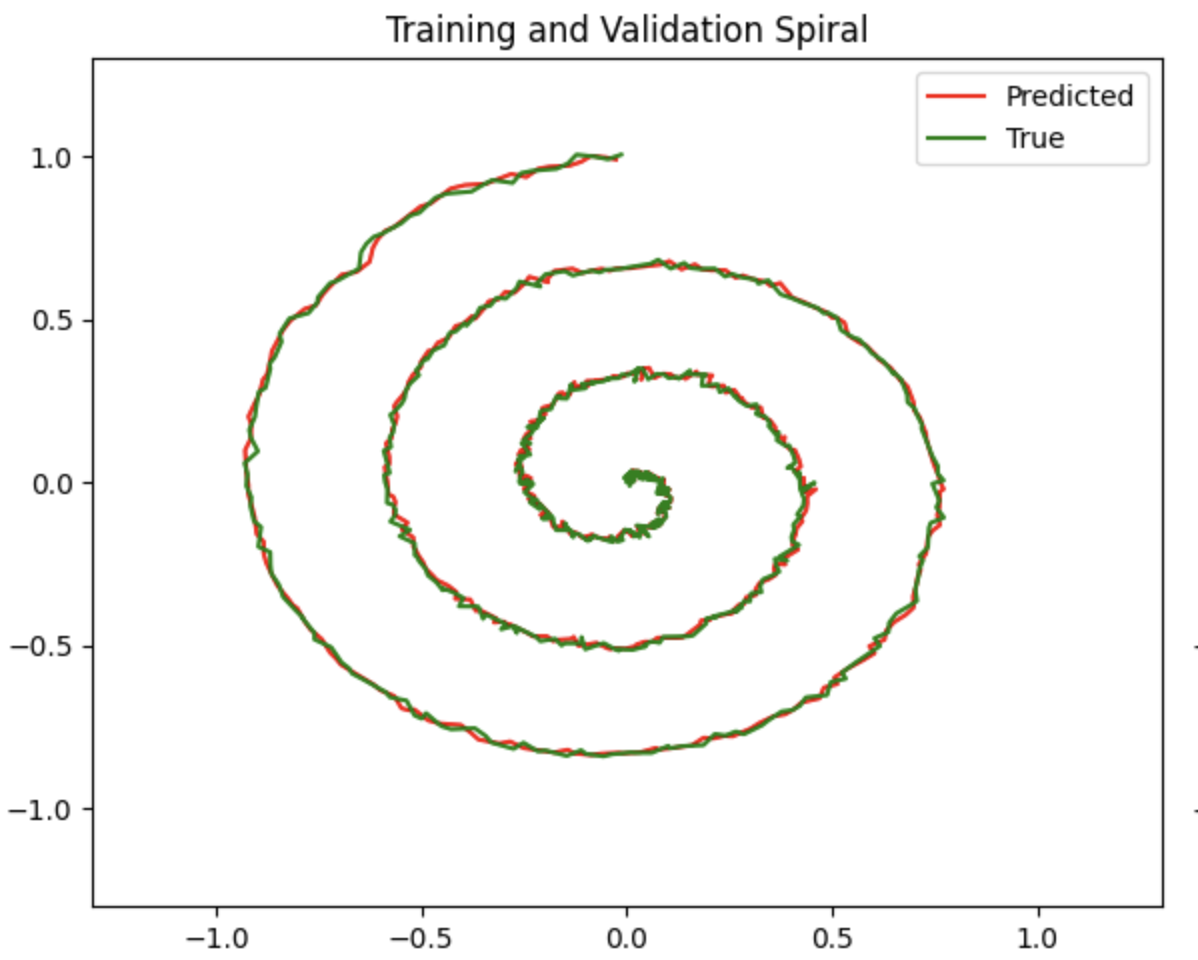
\includegraphics[width=\linewidth]{img/lnn_training_validation_spiral_epoch_2000.png}
        \caption{Epoch 2000}
        \label{fig:lnn_training_validation_spiral_epoch_2000}
    \end{subfigure}
    \caption{LLN predicted vs true spiral trajectories across training: early, mid, and final epochs (denormalised training and validation spiral)}
    \label{fig:lnn_spiral_progression_grid}
\end{figure}

\subsection*{Observed Patterns Across Training Runs}
The number of internal steps in the membrane integration process (\textbf{ODE unfolding depth}) contributed significantly to trajectory stability. Deeper unfolding improved smoothness, but with diminishing returns. The architectures' fixed wiring helped constrain overfitting and contributed to better generalisation than a fully connected architecture. Notably, runs with different initialisations showed \textbf{performance variations} in loss curves and convergence speed, indicating sensitivity to initial wiring or parameter seeds.

Despite simpler architectures having shorter training times (e.g. LSTMs), LLN's had superior interprebility and stability in capturing the underlying continuous structure of the problem.

Although trained on fixed-length input windows, models were evaluated on full-sequence inference without autoregressive rollouts. This mismatch is empirically validated to yield stable and accurate predictions on smooth trajectories.